\documentclass[10pt,twoside,cucitura]{toptesi}
\usepackage{lipsum}
\usepackage{hyperref}
\usepackage{tabularx}
\usepackage{framed}
\usepackage{amsmath}
\usepackage{svg}
\usepackage{graphicx}
\usepackage{float}
\usepackage{array}

\hypersetup{%
    pdfpagemode={UseOutlines},
    bookmarksopen,
    pdfstartview={FitH},
    colorlinks,
    linkcolor={blue},
    citecolor={red},
    urlcolor={blue}
  }

\usepackage[utf8]{inputenc}
\usepackage[T1]{fontenc}\usepackage{lmodern}

\ateneo{ITST J.F. Kennedy}
\nomeateneo{Pordenone}
\FacoltaDi{Specializzazione Informatica}
\titolo{Lupus in Tabula}
\sottotitolo{Limiti della Prima Forma Normale e NoSQL}

\candidato{\tabular{@{}c@{}}Edoardo \textsc{Morassutto}\\Quinta C IA\endtabular}

\sedutadilaurea{\textsc{Anno~scolastico} 2015-2016}
\logosede{icon}

\newcommand{\role}[9]{
\begin{framed}
	\def\arraystretch{0.8}
	\begin{tabularx}{0.75\textwidth}{rX rl}
		ID			& #1 & Priorità		& #5 \\
		Nome		& #2 & Debug		& #6 \\
		Mana		& #3 & Enabled		& #7 \\
		Squadra		& #4 & Chat			& #8 \\
	\end{tabularx}
	%\vspace*{0.07cm}
	\\
	#9
\end{framed}
}

\newcommand{\gamestatus}[3]{
	\textbf{#1}: \textbf{\texttt{#2}}$\quad$ #3
}

\newcommand{\apicode}[3]{
	\texttt{#1} & \texttt{#2} & #3 \\
}

\newcommand{\eventcode}[4]{
	\textbf{#1}: \textbf{\texttt{#2}}$\quad$ #3 
	\vspace{0.1cm}
	\\
	Dati registrati dell'evento:\\
	\begin{tabular}{ll}
		#4
	\end{tabular}
	\vspace{0.2cm}
}

\begin{document}

\frontespizio

\sommario
\emph{Lupus in Tabula} è un gioco di ruolo complesso nel quale i giocatori interpretano dei personaggi e devono raccontare una storia cercando di far vincere la propria squadra. Il gioco, spesso noto anche come Mafia\cite{wiki:mafia}, si basa sul riuscire a dedurre il ruolo degli altri giocatori per capire da chi è composta la propria squadra. 

In questo documento è stato analizzato il problema di modellare i dati delle partite e di creare un server che permettesse a molti utenti di giocare in contemporanea. Durante lo sviluppo ci sono state delle difficoltà riguardo la memorizzazione di alcuni dati delle partite che sono stati in parte risolti.

Il documento è stato diviso in due parti, la prima è un'analisi completa dell'applicazione trattando nel dettaglio ogni aspetto sia progettuale che implementativo, la seconda invece, dopo un'introduzione alle forme normali, tratta delle problematiche incontrate e di alcune delle possibili soluzioni.

Durante lo sviluppo di un database \emph{relazionale} è bene cercare di rispettare le \emph{forme normali}. Una forma normale è un'insieme di regole che evitano che in una base di dati ci sia  ridondanza o inconsistenza.

In questa trattazione si esaminerà uno scenario in cui un semplice database relazionale in prima forma normale non è sufficiente a modellare il problema e si rende necessaria una diversa implementazione.

L'applicazione è stata completata ed è disponibile su \url{https://lupus.serben.tk}, tutto il sorgente è pubblico ed accessibile su \url{https://github.com/lupus-dev/lupus}.

\indici

\mainmatter

%%%%%%%%%%%%%%%%%%%%%%%%%%%%%%%%%%%%%%%%%%%%%%%%%%%%%%%
%                  PARTE UNO                          %
%%%%%%%%%%%%%%%%%%%%%%%%%%%%%%%%%%%%%%%%%%%%%%%%%%%%%%%
\part{Lupus in Tabula}


\chapter{Introduzione generale}

\section{Descrizione del gioco}
Lupus in Tabula è un gioco di ruolo per, normalmente, 7 o più giocatori. Il narratore, che giocando senza computer, è un giocatore speciale che racconta una storia. La storia viene sviluppata da tutti i giocatori che, compiendo delle azioni, comportano dei cambiamenti nella vicenda, per esempio uccidendo dei personaggi o facendoli risorgere.

I giocatori sono divisi in due o più gruppi, esistono sempre le fazioni dei \emph{lupi} e dei \emph{contadini} alle quali può aggiungersi quella dei \emph{criceti mannari} ed altre. Quando la partita finisce solo una di queste squadre vince.

Lo scopo della squadra dei \emph{lupi} è quello di sbranare tutti gli altri giocatori, mentre quello dei \emph{contadini} è di individuare ed uccidere tutti i \emph{lupi}.

La partita si alterna di giorni e di notti, durante ogni notte tutta la squadra dei lupi deve scegliere un bersaglio (solitamente un contadino) che quella notte verrà sbranato. Durante il giorno, invece, ogni giocatore deve votare chi, secondo lui, mandare al rogo. Questo è l'unico modo per i contadini di uccidere i vari lupi che si aggirano nel villaggio. A questa votazione partecipano anche i lupi che cercheranno ovviamente di non farsi votare.

Per rendere il gioco più dinamico vengono inseriti tra i giocatori alcuni ruoli speciali. Per esempio un \emph{veggente} è un contadino che, durante la notte, può scegliere un giocatore vivo e, tramite consultazione della palla di cristallo, sapere se ha un'anima buona oppure cattiva. Ogni ruolo infatti, oltre ad essere di una certa squadra, ha anche delle caratteristiche extra come il \emph{mana}, che può essere buono oppure cattivo. Normalmente (ma non necessariamente) i giocatori nella squadra dei lupi hanno mana cattivo mentre quelli nella squadra dei contadini ce l'hanno buono.

Ogni giocatore, in generale, conosce solo il proprio ruolo e deve dedurre quello degli altri giocatori; ci possono essere dei casi in cui qualche giocatore conosce il ruolo esatto di qualcun altro. Per esempio ogni lupo conosce esattamente quali sono i suoi compagni di squadra.

Quanto un giocatore muore in una partita normale è il narratore ad annunciarlo, in questa implementazione è presente un giornale nel quale viene scritto il nome dei giocatori che sono morti.

Affinché una partita termini correttamente deve verificarsi almeno una delle seguenti condizioni:

\begin{itemize}
	\item Tutti i giocatori sono morti
	\item Almeno una fazione ha vinto
	\begin{itemize}
		\item Lupi: Il numero di lupi è maggiore o uguale al numero di contadini
		\item Contadini: Il numero di lupi è zero
	\end{itemize}
\end{itemize}

\section{Ruoli}
Ad ogni giocatore viene assegnato dal sistema uno ed un solo ruolo, quindi il giocatore saprà anche la sua fazione e il suo mana. 

Ogni ruolo, oltre al nome ha anche alcune proprietà aggiuntive:

\begin{itemize}
	\item Mana: indica se il giocatore agirà come malintenzionato oppure come una brava persona
	\item Nome identificativo: nome unico che identifica il ruolo
	\item Priorità: serve per stabilire un ordine nell'esecuzione delle azioni
	\item Debug: alcuni ruoli sono accessibili solo dagli sviluppatori e sono marcati come \emph{debug}
	\item Enabled: È possibile disattivare alcuni ruoli con questa proprietà
	\item Chat: alcuni ruoli hanno dei canali di comunicazione dedicati
	\item Gen*: parametri aggiuntivi per la generazione automatica dei ruoli, come numero minimo e massimo di occorrenze del ruolo, probabilità, ecc...
\end{itemize}

\subsection{Ruoli comuni}

I ruoli che normalmente vengono usati in una partita di Lupus in Tabula sono:

\role{Lupo}{Lupo}{Cattivo}{Lupi}{100}{no}{sì}{Lupi}{Durante la notte i \emph{lupi} votano chi eliminare, se almeno il 50\%+1 dei \emph{lupi} vivi votano la stessa persona, questa è una candidata a morire}

\role{Guardia}{Guardia}{Buono}{Contadini}{10000}{no}{si}{}{Durante la notte la \emph{guardia} può scegliere di proteggere una persona, se i \emph{lupi} quella notte decidessero di ucciderla, essa non muore}

\role{Medium}{Medium}{Buono}{Contadini}{150}{no}{si}{}{Il \emph{medium} durante la notte può scegliere di guardare un giocatore morto, lui saprà se quel giocatore aveva un mana buono o cattivo}

\role{Paparazzo}{Paparazzo}{Buono}{Contadini}{1000}{no}{si}{}{Il \emph{paparazzo} durante la notte sceglie una persona da pedinare, vengono riportati sul giornale della mattina seguente tutti i giocatori che hanno visitato il personaggio \textsl{paparazzato}}

\role{Criceto mannaro}{Criceto mannaro}{Cattivo}{Criceti}{10000}{no}{si}{}{\'E un giocatore normale, senza poteri speciali. Se la partita termina e lui è ancora vivo allora vince solo lui e non la sua fazione}

\role{Assassino}{Assassino}{Cattivo}{Contadini}{10}{no}{si}{}{L'\emph{assassino} una sola volta nella partita può scegliere una persona e ucciderla}

\role{Massone}{Massone}{Buono}{Contadini}{10000}{no}{si}{Massoni}{I \emph{massoni} non hanno poteri però hanno una chat dedicata e quindi si conoscono tra loro}

\role{Contadino}{Contadino}{Buono}{Contadini}{10000}{no}{si}{}{I \emph{contadini} non hanno poteri\dots}

\role{Pastore}{Pastore}{Buono}{Contadini}{50}{sì}{si}{}{I \emph{pastori} possono scegliere di sacrificare delle pecore per salvare dei giocatori dalle grinfie dei lupi}

\role{Sindaco}{Sindaco}{Buono}{Contadini}{10000}{no}{si}{}{Il \emph{sindaco} è un contadino che non può essere messo al rogo nella votazione diurn}

\chapter{Analisi}

\section{Analisi del problema}
È necessario sviluppare un sistema robusto che gestisce gli utenti e le partite di Lupus in Tabula.

Il sistema deve essere in grado di sopportare un numero crescente di giocatori e un numero molto elevato di partite, deve essere in grado di scalare ottimalmente con le richieste. La base di dati deve essere sviluppata in modo da garantire un funzionamento efficiente e una robustezza dei dati.

I dati identificativi degli utenti devono essere conservati in modo sicuro, è necessario proteggere le credenziali di accesso tramite moderni sistemi di \emph{hashing}.

È necessario fare molta attenzione ai privilegi degli utenti, proteggendo le risorse che non sono accessibili. Per esempio è opportuno evitare che gli utenti possano vedere, entrare o modificare le partite alle quali gli è stato negato il permesso.

Le chiavi interne del database non sono visibili agli utenti, delle chiavi alternative non numeriche sono visualizzate al loro posto. Per esempio le partite non vengono identificate (lato utente) da un intero progressivo ma da un \emph{nome breve}, una sequenza di caratteri che rispetta la seguente \texttt{regex}: \texttt{[a-zA-Z][a-zA-Z0-9]\{0,9\}}. Deve essere lungo da 1 a 10 caratteri \texttt{ASCII}, il primo carattere deve essere una lettera e deve essere unico nel suo contesto.

\section{Stuttura dei componenti}
Ogni utente registrato nel sistema può giocare alle partite create dagli altri giocatori oppure può crearne di nuove. Per creare delle partite l'utente deve creare delle stanze, dei raggruppamenti di zero, una o più partite.

Una stanza appartiene ad uno ed un solo utente che ha poteri amministrativi su questa, solo lui può creare una nuova partita in quella stanza. Ogni stanza viene identificata da un \emph{nome breve} univoco e non modificabile ed ha una breve descrizione. In una stanza ci può essere al più una parita in corso.

Quando un utente possiede una stanza libera (senza partite in corso), può decidere di creare una nuova partita, questa viene identificata da un \emph{nome breve} univoco all'interno della stanza ma non globalmente e non modificabile. La partita ha anche una breve descrizione.

Gli altri utenti possono entrare nella partita solo se hanno i permessi per farlo, ogni partita infatti condivide i permessi della stanza a cui appartiene, per esempio se la stanza è protetta da delle liste di accesso (\texttt{ACL}), solo gli utenti specificati possono accedervi.

Una partita è composta da una serie di giocatori, degli utenti a cui è stato assegnato un ruolo (eventualmente non definito). Appena un giocatore entra nella partita (e questa non è iniziata) gli viene assegnato un ruolo non definito (\texttt{unknown}). Appena il numero di giocatori raggiunge il valore specificato dall'amministratore vengono generati i ruoli esatti dei giocatori. I ruoli possono essere generati in due modi: manualmente secondo precise impostazioni dell'amministratore oppure automaticamente specificando solo quali ruoli usare.

Ogni utente può giocare anche a diverse partite in contemporanea, in accordo con i limiti imposti dal suo livello. Ogni utente infatti ha un livello che limita le sue possibilità di gioco, come il numero di partite contemporanee, il numero di stanze pubbliche e private.

Il livello di un giocatore è sempre crescente, si può venire declassati solo dall'amministratore del server. Il livello viene stabilito tramite un valore detto \emph{karma} che rappresenta un'indicazione del tempo di gioco dell'utente. Si guadagnano punti karma giocando partite, vincendo partite o invitando altri giocatori. Quando il karma raggiunge un valore sufficientemente alto viene aumentato il livello dell'utente. 

Per poter usare le funzionalità in beta è necessario possedere un livello sufficientemente alto.

Il livello di un utente è visibile nella pagina dell'utente e in ogni partita viene evidenziato. I possibili livelli sono:

\begin{table}
	\begin{tabular}{|c|c|c|c|c|c|c|}
		\hline
		& \textbf{Nome} & \textbf{Karma} & \textbf{Partite parallele} & \textbf{Stanze} & \textbf{Stanze private} & \textbf{BETA} \\
		\hline
		1 & Neofita 	 & 0    &   3 &   1 &   0 & no \\
		2 & Principiante & 25   &   5 &   1 &   0 & no \\
		3 & Gamer        & 50   &   5 &   3 &   1 & no \\
		4 & Esperto      & 100  &   5 &   5 &   3 & no \\
		5 & Maestro      & 200  &   7 &   5 &   5 & no \\
		6 & ProGamer     & 500  &  10 &  10 &   5 & no \\
		7 & Stratega     & 2000 &  15 &  10 &  10 & si \\
		8 & Generale     & 5000 &  50 & 100 &  10 & si \\
		9 & Guru         & 10000& 100 & 100 & 100 & si \\
		10 & GameMaster   & $\infty$ & 1000 & 1000 & 1000 & si \\
		\hline
	\end{tabular}
	\caption{Livelli degli utenti}
	\label{tab:livelli}
\end{table}

Giocando è anche possibile sbloccare degli obiettivi che arricchiscono il profilo del giocatore, un badge verrà infatti visualizzato nella pagina dell'utente appena compie un'azione memorabile. Il valore di \emph{difficoltà} serve per ordinare gli obiettivi, non necessariamente indica la difficoltà.

\begin{table}
	\centering
	\begin{tabular}{|L{3cm}|L{4cm}|L{5.6cm}|C{1.7cm}|}
		\hline
		\textbf{Codice} & \textbf{Nome} & \textbf{Descrizione} & \textbf{Difficoltà} \\
		\hline
		AtLeast5Games & Appena iniziato & Gioca almeno 5 partite & 10 \\
		AtLeast20Games & Iniziamo a ragionare... & Gioca almeno 20 partite & 11 \\
		AtLeast50Games & Esperto del mestiere & Gioca almeno 50 partite & 12 \\
		AtLeast100Games & Saggio del villaggio & Gioca almeno 100 partite & 13 \\
		
		AtLeast5Wins & Primi successi & Vinci almeno 5 partite & 20 \\
		AtLeast20Wins & Hai capito le regole & Vinci almeno 20 partite & 21 \\
		AtLeast50Wins & Pericolo pubblico & Vinci almeno 50 partite & 22 \\
		AtLeast100Wins & Stratega professionista & Vinci almeno 100 partite & 23 \\
		\hline
	\end{tabular}
	\caption{Obiettivi sbloccabili}
	\label{tab:obiettivi}
\end{table}

\section{Progettazione della base di dati}
Come analizzato nella Parte II [\ref{sec:soluzione}] il database è stato diviso in due parti, una relazionale e una \texttt{NoSQL}. In merito alla parte relazionale è qui proposto uno schema Entità-Relazione.

Alcuni attributi sono stati mantenuti dal passaggio dalla prima versione del Database (senza NoSQL) a quella più recente. In particolare tutti gli attributi che non rispettavano la Prima Forma Normale sono stati lasciati ed ora sono facoltativi (se lasciati a \texttt{NULL} viene usata la versione in NoSQL).

Tutto ciò sia per retrocompatibilità che per garantire il funzionamento della piattaforma anche in eventuali servizi di hosting che non supportano NoSQL.

\subsection{Schema concettuale}
Nello schema in figura \ref{fig:er} sono riportate tutte le entità e le relazioni che compongono la base di dati. In ogni entità sono anche elencati tutti gli attributi che la compongono, comprese le chiavi primarie ed eventuali vincoli di unicità.

I campi marcati con una \texttt{x} sono i campi interessati dalla ristrutturazione tramite NoSQL. Fare riferimento alla descrizione presente nella Parte II, in particolare [\ref{sec:soluzione}].

% quick layout fix
\newpage

\begin{figure}[H]
	\centering
	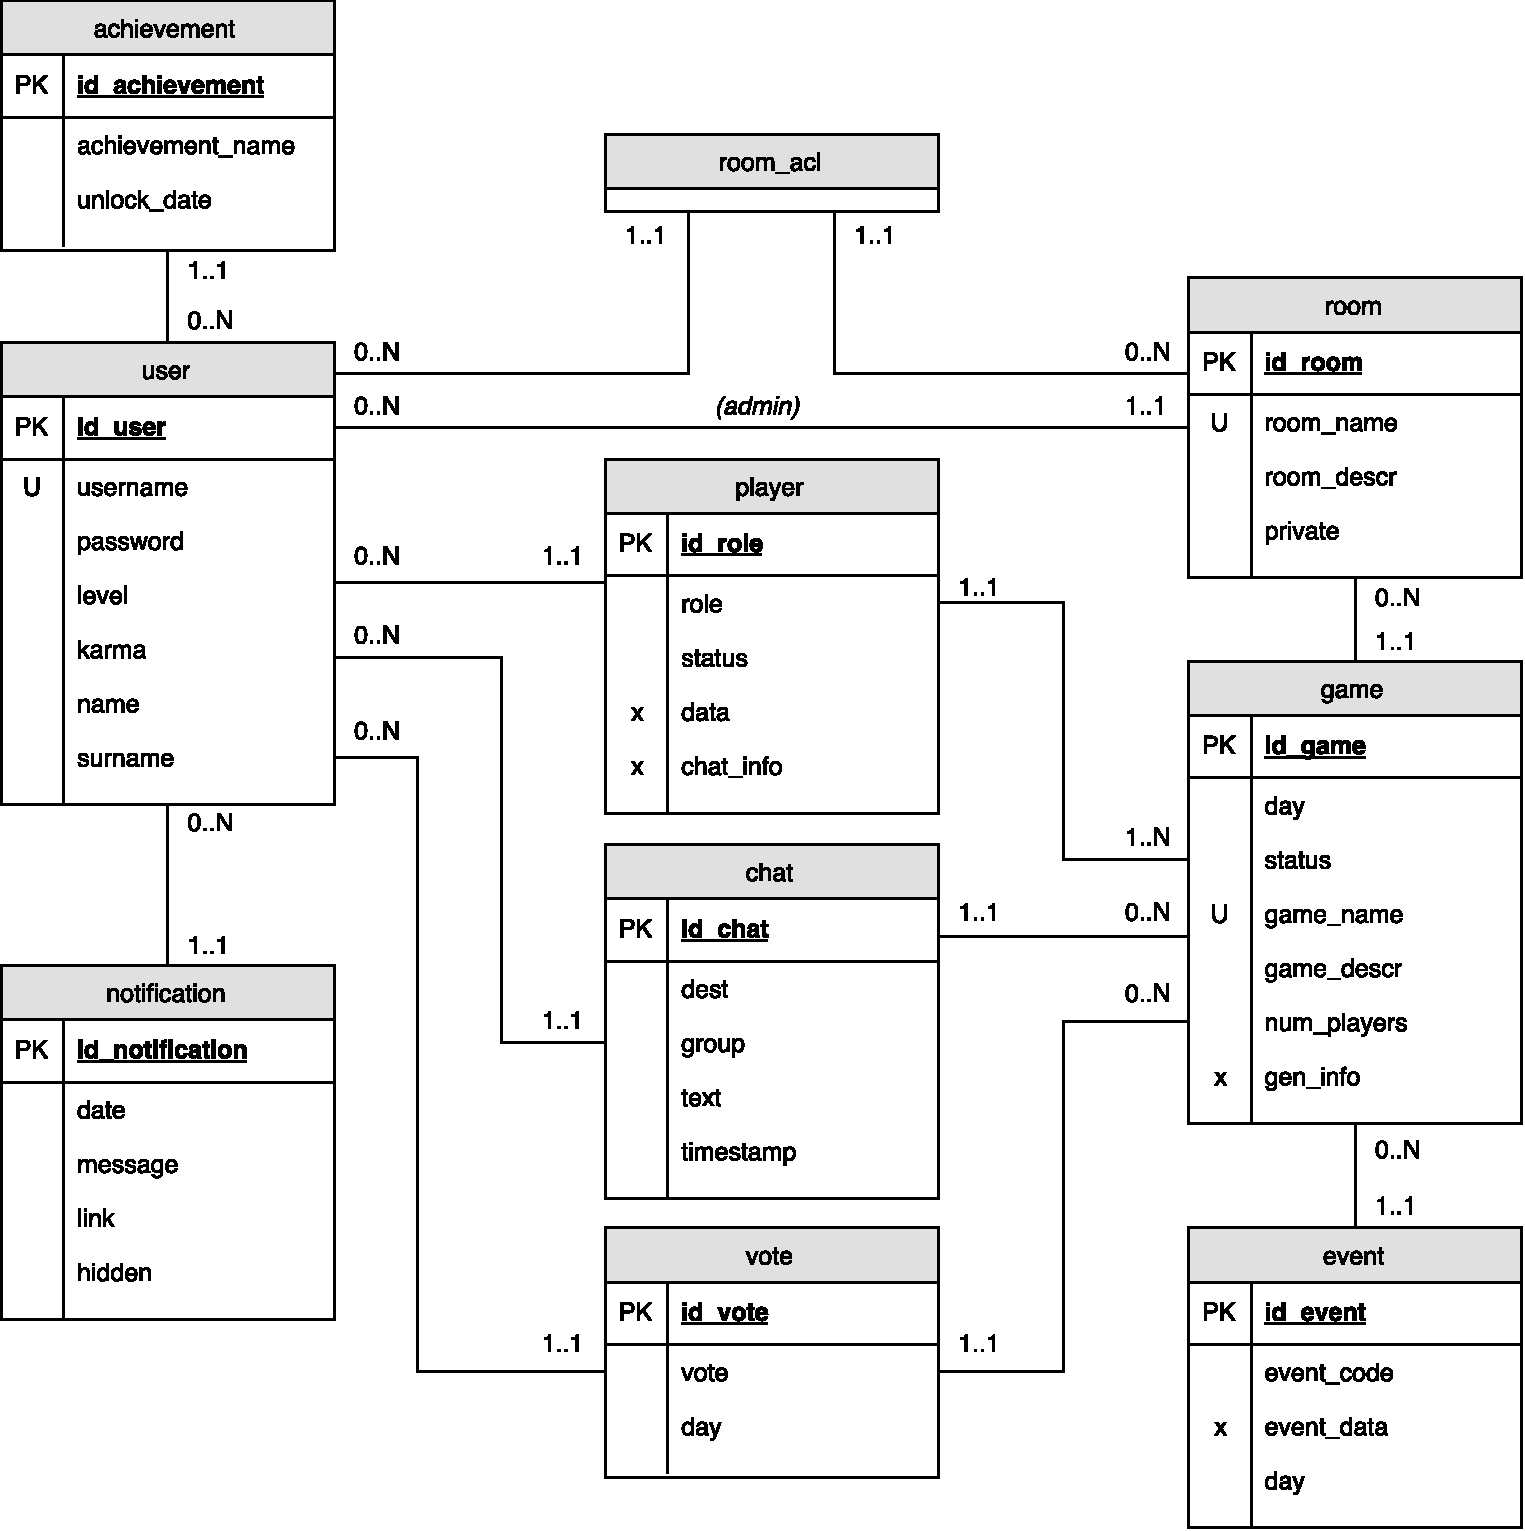
\includegraphics[width=\textwidth]{ER.pdf}
	\caption{Diagramma Entità-Relazione della base di dati}
	\label{fig:er}
\end{figure}



\subsection{Schema logico}
Vengono qui riportate, in modo sintetico le definizioni di tutte le tabelle che compongono la base di dati. Le chiavi primarie sono \underline{sottolineate}, le chiavi esterne sono in \emph{corsivo} con il relativo riferimento; i campi ristrutturati con NoSQL hanno un asterisco ($^*$).

\begin{itemize}
	\item \texttt{user(\underline{id\_user}, username, password, level, karma, name, surname)}
	\item \texttt{room(\underline{id\_room}, \emph{id\_admin}\extkey{user.id\_user}, room\_name, room\_descr, private)}
	\item \texttt{game(\underline{id\_game}, \emph{id\_room}\extkey{room.id\_room}, day, status, game\_name, game\_descr, \\num\_players, gen\_info$^*$)}
	\item \texttt{player(\underline{id\_role}, \emph{id\_game}\extkey{game.id\_game}, \emph{id\_user}\extkey{user.id\_user}, role, status, data$^*$, \\chat\_info$^*$)}
	\item \texttt{chat(\underline{id\_chat}, \emph{id\_game}\extkey{game.id\_game}, \emph{id\_user\_from}\extkey{user.id\_user}, dest, group, text, \\timestamp)}
	\item \texttt{vote(\underline{id\_vote}, \emph{id\_game}\extkey{game.id\_game}, \emph{id\_user}\extkey{user.id\_user}, vote, day)}
	\item \texttt{event(\underline{id\_event}, \emph{id\_game}\extkey{game.id\_game},  event\_code, event\_data$^*$, day)}
	\item \texttt{notification(\underline{id\_notification}, \emph{id\_user}\extkey{user.id\_user}, date, message, link, hidden)}
	\item \texttt{achievement(\underline{id\_achievement}, \emph{id\_user}\extkey{user.id\_user}, achievement\_name, unlock\_date)}
	\item \texttt{room\_acl(\underline{\emph{id\_room}}\extkey{room.id\_room}, \underline{\emph{id\_user}}\extkey{user.id\_user})}
\end{itemize}

\subsection{Descrizione delle entità}
Vengono qui riportate le descrizioni dettagliate di tutte le tabelle presenti nella base di dati. Anche gli attributi sono elencati ed analizzati, con particolare riferimento alle varie caratteristiche di questi. Nella varie tabelle che seguono vengono usate delle abbreviazioni per snellire la trattazione. In particolare riguardo i vincoli le varie sigle significano:

\begin{itemize}
	\item \textbf{P}: chiave primaria
	\item \textbf{E}: chiave esterna
	\item \textbf{U}: vincolo di unicità
	\item \textbf{X}: attributo ristrutturato nel NoSQL
	\item \textbf{N}: attributo opzionale (\texttt{NULL})
\end{itemize}

È possibile trovare anche la combinazione di queste lettere.

Nella colonna relativa al dominio viene indicato il tipo di dato dell'attributo, se maiuscolo è da riferirsi ad uno dei tipi predefiniti. In caso di chiavi esterne in questa colonna viene indicato l'attributo di ``chiave primaria'' collegato.

\subsubsection{Tabella \texttt{user}}

Questa tabella contiene le informazioni personali di ogni utente, compreso username e password. Ogni utente possiede un livello numerico intero e un livello di karma, sempre intero. Nella tabella sono anche memorizzati il nome e il cognome dell'utente.

Per la gestione della password è stato adottato un metodo particolare per garantire il funzionamento anche su sistemi datati o privi della libreria \texttt{crypto}. 

Se il server PHP supporta le funzioni \texttt{password\_hash} e \texttt{password\_verify} allora vengono usate quelle, altrimenti viene usata la funzione \underline{non sicura} SHA-1.

La funzione \texttt{password\_hash} cifra la password utilizzando l'algoritmo \texttt{CRYPT\_BLOWFISH} che viene ripetuto 10 volte e viene utilizzato un \emph{salt} crittograficamente sicuro. Questo algoritmo è sufficientemente lento da evitare attacchi di tipo \emph{brute-force} e l'utilizzo del salt evita che le password vengano ricavate facilmente attraverso tabelle di lookup.

La funzione \texttt{password\_verify} effettua l'hash della password inviata in chiaro utilizzando gli stessi parametri di \texttt{password\_hash} ed effettua un confronto tra le due stringhe non vulnerabile a degli attacchi \emph{timed-based}.

\attributi{user}{
	id\_user & P & INT & Identificativo dell'utente \\
	username & U & VARCHAR(10) & Username dell'utente \\
	password &   & VARCHAR(255) & Hash della password dell'utente \\
	level    &   & INT & Numero del livello dell'utente, fare riferimento alla tabella [\ref{tab:livelli}] \\
	karma    &   & INT & Punti karma dell'utente \\
	name     &   & VARCHAR(50) & Nome dell'utente \\
	surname  &   & VARCHAR(50) & Cognome dell'utente \\
}


\subsubsection{Tabella \texttt{room}}

Ogni stanza ha un identificativo univoco \texttt{id\_room}, nascosto al pubblico che identifica la stanza all'interno del database. Al pubblico la stanza è identificata con un nome \texttt{room\_name} il quale è unico. Ogni stanza ha anche una descrizione \texttt{room\_descr} che rappresenta il titolo della stanza. 

Ogni stanza contiene l'identificativo dell'utente amministratore della stanza \texttt{id\_admin}. 

Il campo \texttt{private} indica se la stanza è pubblica o privata, secondo le specifiche in [\ref{sec:visibilita}].

\attributi{room}{
	id\_room   & P & INT & Identificativo della stanza \\
	id\_admin  & E & user.id\_user & Identificativo dell'utente a cui appartiene la stanza \\
	room\_name & U & VARCHAR(10) & Nome identificativo della stanza \\
	room\_descr &   & VARCHAR(50) & Descrizione della stanza \\
	private    &   & INT & Grado di visibilità della stanza \\
}


\subsubsection{Tabella \texttt{game}}

Ogni partita è identificata all'interno del database con un identificativo unico \texttt{id\_game}. Ogni partita è identificata all'esterno con un \emph{nome breve} unico all'interno della stessa stanza (\texttt{game\_name}), inoltre ha una descrizione che rappresenta il titolo della partita \texttt{game\_descr}.

Ogni partita è contenuta all'interno della stanza con id \texttt{id\_room}. I campi \texttt{day} e \texttt{status} sono informazioni utili della partita, l'istante temporale del gioco e lo stato della partita.

Il numero di giocatori è memorizzato nel campo \texttt{num\_players} per eseguire velocemente alcune query. Le informazioni per generare la partita vengono memorizzate nel database NoSQL, in precedenza erano memorizzate come JSON nel campo \texttt{gen\_info}.

% quick layout fix
\newpage

\attributi{game}{
	id\_game    & P & INT & Identificativo della partita \\
	id\_room    & E & room.id\_room & Identificativo della stanza associata \\
	day         &   & INT & Giorno in cui si trova la partita. Fare riferimento a \ref{sec:tempo} \\
	status      &   & INT & Stato in cui si trova la partita. Fare riferimento a \ref{sec:statoPartita} \\
	game\_name  & U & VARCHAR(10) & Nome breve della partita. Deve essere unico all'interno della stanza \\
	game\_descr &   & VARCHAR(50) & Descrizione della partita \\
	num\_players &  & INT & Numero di giocatori nella partita \\
	gen\_info  & XN & VARCHAR(500) & Informazioni per generare la partita \\
}


\subsubsection{Tabella \texttt{player}}

In questa tabella sono memorizzati i ruoli dei giocatori interni ad una partita. 

Ogni riga è identificata da un campo \texttt{id\_role} non pubblico. Ogni ruolo è interno alla partita \texttt{id\_game} e relativo all'utente \texttt{id\_user}. Il ruolo dell'utente è memorizzato nella stringa \texttt{role} la quale identifica un ruolo nella cartella dei ruoli. Per approfondire il significato di questa stringa fare riferimento a [\ref{sec:polimorfismo}].

Il campo \texttt{status} indica lo stato dell'utente (vivo/morto/espulso). Alcuni ruoli potrebbero richiedere di memorizzare delle informazioni aggiuntive, il campo \texttt{data} (che viene memorizzato nel NoSQL) contiene dei dati salvati da un ruolo. Un giocatore ha anche memorizzato alcune informazioni sulle sue chat, per sapere quali sono i messaggi che non ha ancora letto.

\attributi{player}{
	id\_role   & P & INT & Identificativo del giocatore \\
	id\_game   & E & game.id\_game & Identificativo della partita associata \\
	id\_user   & E & user.id\_user & Identificativo dell'utente associato \\
	role       &   & VARCHAR(50) & Nome identificativo del ruolo corrispondente, fare riferimento a [\ref{sec:polimorfismo}]. \\
	status     &   & INT & Stato dell'utente nella partita, fare riferimento a [\ref{sec:statoGiocatore}] \\
	data       & XN & VARCHAR(500) & Dati aggiuntivi del ruolo \\
	chat\_info & XN & VARCHAR(500) & Informazioni sulle chat del giocatore \\
}


\subsubsection{Tabella \texttt{chat}}

In questa tabella vengono memorizzati i messaggi delle varie chat. Ogni messaggio è identificato all'interno del database da \texttt{id\_chat} ed è relativo ad una singola partita (\texttt{id\_game}).

Il mettente del messaggio è \texttt{id\_user\_from} cioè l'identificativo dell'utente che ha inviato il messaggio. Il destinatario \texttt{dest} è un numero intero che può rappresentare vari identificativi, in base a \texttt{group} il destinatario può essere un utente, il pubblico, una chat privata, ecc...

Il testo del messaggio è \texttt{text} il quale non può essere più lungo di 200 caratteri e viene eseguito l'\emph{escape} sia per il database che per il JavaScript.

\newpage

\attributi{chat}{
	id\_chat   & P & INT & Identificativo del messaggio \\
	id\_game   & E & game.id\_game & Partita associata \\
	id\_user\_from & E & user.id\_user & Utente mittente del messaggio \\
	dest &   & INT & Destinatario del messaggio \\
	group &   & INT & Gruppo di destinazione del messaggio \\
	text &  & VARCHAR(200) & Testo del messaggio \\
	timestamp &  & TIMESTAMP & Data e ora di invio del messaggio \\
}


\subsubsection{Tabella \texttt{vote}}

In questa tabella vengono memorizzati i voti degli utenti. Ogni voto è identificato tramite il campo \texttt{id\_vote}, il quale rimane nascosto all'esterno del database. Ogni voto è specifico della partita \texttt{id\_game} nel momento \texttt{day} e appartiene all'utente \texttt{id\_user}. 

Il voto è \texttt{vote} il quale può essere l'identificativo di un utente, un voto \emph{nullo} o altro. 

\attributi{vote}{
	id\_vote & P & INT & Identificativo della votazione \\
	id\_game & E & game.id\_game & Identificativo della partita associata \\
	id\_user & E & user.id\_user & Identificativo del giocatore associato \\
	vote &  & INT & Voto dell'utente \\
	day &  & INT & Giorno della partita in cui vale la votazione \\
}


\subsubsection{Tabella \texttt{event}}

In questa tabella vengono memorizzati gli eventi delle partite. Ogni evento è identificato dal campo \texttt{id\_event} e appartiene alla partita \texttt{id\_game} ed è specifico del giorno \texttt{day} secondo le specifiche in [\ref{sec:tempo}].

Il tipo di evento che si è verificato è memorizzato in \texttt{event\_code} secondo i codici descritti in [\ref{sec:codiciEventi}]. Il campo dei dati dell'evento è memorizzato nel database NoSQL e in precedenza era salvato come JSON in \texttt{event\_data}.

\attributi{event}{
	id\_event & P & INT & Identificativo dell'evento \\
	id\_game  & E & game.id\_event & Partita associata all'evento \\
	event\_code &  & INT & Codice dell'evento, fare riferimento a [\ref{sec:codiciEventi}] \\
	event\_data & XN & VARCHAR(500) & Dati dell'evento \\
	day &  & INT & Giorno della partita \\
}

\newpage

\subsubsection{Tabella \texttt{notification}}

In questa tabella sono memorizzate tutte le notifiche di un utente. Le notifiche cancellate non vengono rimosse ma semplicemente marcate come lette. Ogni notifica viene identificata dal campo \texttt{id\_notification} ed appartiene all'utente \texttt{id\_user}.

Il testo del messaggio si trova nel campo \texttt{message} ed avrà un collegamento \texttt{link}, il quale è il percorso assoluto senza \texttt{basePath} (vedi capitolo [\ref{sec:pagineWeb}]). La notifica viene nascosta tramite il parametro \texttt{hidden}.

Nel testo della notifica è possibile inserire dell'HTML per aggiungere dello stile.

\attributi{notification}{
	id\_notification & P & INT & Identificativo della notifica \\
	id\_user & E & user.id\_user & Utente a cui appartiene la notifica \\
	date &  & TIMESTAMP & Data di generazione della notifica \\
	message & & VARCHAR(200) & Testo della notifica \\
	link & & VARCHAR(200) & Collegamento alla notifica \\
	hidden & & TINYINT & Booleano che indica se la notifica è stata nascosta \\
}


\subsubsection{Tabella \texttt{achievement}}

Gli obiettivi sbloccati dagli utenti sono memorizzati in questa tabella. Ogni obiettivo sbloccato viene identificato dal campo \texttt{id\_achievement}. Per riconoscere l'obiettivo viene usato il campo \texttt{achievement\_name} che contiene il nome identificativo dell'obiettivo, come descritto nella tabella [\ref{tab:obiettivi}].

\attributi{achievement}{
	id\_achievement & P & INT & Identificativo dell'obiettivo sbloccato \\
	id\_user & E & user.id\_user & Utente che ha sbloccato l'obiettivo \\
	achievement\_name & & VARCHAR(50) & Nome identificativo dell'obiettivo \\
	unlock\_date & & TIMESTAMP & Data di sblocco dell'obiettivo \\
}


\subsubsection{Tabella \texttt{room\_acl}}

Le stanze che sono state impostate private con controllo degli accessi utilizzano questa tabella per sapere quali sono gli utenti autorizzati. La tabella contiene due campi che formano la chiave primaria: \texttt{id\_room} e \texttt{id\_user}.

\attributi{room\_acl}{
	id\_room & PE & room.id\_room & Identificativo della stanza \\
	id\_user & PE & user.id\_user & Identificativo dell'utente \\
}

\newpage

\section{Codici utilizzati}
Nel gioco, per alleggerire la base di dati e per snellire il tutto sono state usate delle convenzioni riguardo alcuni codici. Per esempio per evitare di memorizzare un'intera stringa come \texttt{Giorno 4} è stato scelto di memorizzare l'intero 6, mentre per la \texttt{Notte 1} il valore 1.

Questi codici sono qui riportati e descritti e sono modificabili sono andando ad intervenire nella apposite classi dedicate alla sola memorizzazione di queste costanti. Questi valori non sono stati usati semplicemente nel codice ma viene sempre fatto riferimento alle costanti specificate.

\subsection{Tempo del gioco}
\label{sec:tempo}
Come appena preannunciato il tempo di una partita viene semplicemente memorizzato come numero intero secondo la seguente convenzione:

\[
day
\left\{
\begin{aligned}
\text{se}\ day = 0 						&\Rightarrow \text{arrivo al villaggio} \\
\text{se}\ day\ \text{è \emph{pari}}		&\Rightarrow \text{giorno}\ \frac{day}{2}+1 \\
\text{se}\ day\ \text{è \emph{dispari}}	&\Rightarrow \text{notte}\ \frac{day}{2}+1
\end{aligned}
\right.
\]

Il valore di \emph{day} viene memorizzato nella tabella game in quanto si tratta del giorno della partita.

Sono qui riportati degli esempi dei valori che può assumere \emph{day}:

\begin{tabular}{|c|c|}
	\hline
	\textbf{day} & \textbf{valore} \\
	\hline
	0 & Arrivo al villaggio \\
	1 & Notte 1 \\
	2 & Giorno 2 \\
	3 & Notte 2 \\
	4 & Giorno 3 \\
	5 & Notte 3 \\
	6 & Giorno 4 \\
	7 & Notte 4 \\
	\hline
\end{tabular}

\subsection{Stato della partita}
\label{sec:statoPartita}
Ogni partita deve trovarsi in uno stato preciso che indica le condizioni della partita. In particolare è necessario sapere se la partita è già iniziata, se è finita, se ha vinto una certa squadra, se è stata interrotta ecc...

Per rendere più chiaro il valore di questi codici i vari stati delle partite sono stati divisi in alcune fasi: Pre-Partita, In-Partita, Terminata-OK, Terminata-Errore.

\subsubsection{Fase Pre-Partita}
Questa fase è presente solo prima dell'avvio della partita e serve per salvare ed aggiustare i dettagli della partita, come il numero di giocatori, di ruoli, la descrizione, ecc\dots

Questa fase è identificata da codici nell'intervallo:
\[
0 \le x < 100
\]

I codici riconosciuti sono:
\begin{itemize}
	\item \gamestatus{0}{Setup}{Impostazione della partita}
\end{itemize}


\subsubsection{Fase In-Partita}
Questa fase è presente poco prima dell'inizio della partita e durante tutto il corso della partita. 

Viene identificata da codici nell'intervallo:
\[
100 \le x < 200
\]

I codici riconosciuti sono:
\begin{itemize}
	\item \gamestatus{100}{NotStarted}{La partita è attiva e i giocatori possono iniziare ad entrare}
	\item \gamestatus{101}{Running}{La partita è in corso e i giocatori non possono più entrare}
\end{itemize}


\subsubsection{Fase terminata in modo corretto}
Questa fase si verifica quando la partita termina in modo corretto e viene scelta una squadra vincitrice.

I codici che la identificano sono compresi nell'intervallo:
\[
200 \le x < 300
\]

I codici riconosciuti sono:
\begin{itemize}
	\item \gamestatus{200\,+\,y}{Win$y$}{La partita è terminata e ha vinto la squadra $y\ (0\le y < 99)$}
	\item \gamestatus{299}{DeadWin}{La partita è terminata perché tutti i giocatori sono morti}
\end{itemize}



\subsubsection{Fase terminata in modo inaspettato}
Questa fase si verifica quando la partita viene interrotta prima della sua normale fine. In questo caso non viene designato alcun vincitore.

I codici che identificano questa fase sono compresi dall'intervallo:
\[
300 \le x < 400
\]

I codici riconosciuti sono:
\begin{itemize}
	\item \gamestatus{300}{TermByAdmin}{L'amministratore della stanza ha fatto terminare la partita}
	\item \gamestatus{301}{TermBySolitude}{Un numero eccessivo di giocatori hanno abbandonato la partita}
	\item \gamestatus{302}{TermByVote}{\'E stato raggiunto il \emph{quorum} per terminare la partita}
	\item \gamestatus{303}{TermByBug}{Un errore interno del server ha fatto terminare la partita per preservare l'integrità del server}
	\item \gamestatus{304}{TermByGameMaster}{Il GameMaster ha deciso di terminare la partita}
\end{itemize}

\subsection{Codici di risposta delle API}
Le funzioni delle API ritorneranno un codice numerico identificativo del messaggio di errore/successo che la relativa funzione ha avuto. 

I codici sono divisi in gruppi di decine: le unità sono un numero progressivo che identifica la sezione caratterizzata dalle altre cifre del codice.

\resizebox{\textwidth}{!} {
\begin{tabular}{|rl|l|}
\hline
\textbf{\#} & \textbf{Abbreviazione} & \textbf{Descrizione} \\
\hline
\apicode{1}{NotLoggedIn}{L'utente non è connesso e non può accedere a questa risorsa}
\apicode{2}{FatalError}{Un errore grave interno al server può aver compromesso la partita}
\apicode{3}{AccessDenied}{L'utente non ha i permessi per accedere alla risorsa richiesta}
\apicode{4}{NotFound}{La risorsa richiesta non è stata trovata}
\apicode{5}{MissingParameter}{Non è stato specificato un parametro richiesto}
\apicode{6}{MalformedParameter}{Uno dei parametri non ha un formato corretto o è invalido}
\apicode{7}{Done}{La richiesta è stata completata con successo}
\apicode{8}{Fail}{La richiesta non è stata completata a causa di un errore}
\apicode{9}{Found}{La risorsa è stata trovata}
\hline
\apicode{101}{LoginAlreadyDone}{Utente già connesso}
\hline
\apicode{130}{JoinDoneGameStarted}{L'utente è entrato nella partita e questa è iniziata}
\apicode{131}{JoinDoneGameWaiting}{L'utente è entrato nella partita ma questa è in attesa}
\apicode{132}{JoinFailedAlreadyIn}{L'utente era già entrato nella partita}
\apicode{133}{JoinFailedGameClose}{Non sono permessi ingressi}
\apicode{134}{JoinFailedGameFull}{L'utente non è entrato nella partita perché è piena}
\apicode{135}{JoinFailedGamesEnded}{La partità era finita, il giocatore non è entrato}
\hline
\apicode{143}{NewGameAlreadyRunning}{Una partita nella stanza è ancora in corso}
\apicode{144}{NewGameAlreadyExists}{Esiste già una partita con questo nome nella stanza}
\hline
\apicode{152}{StartNotInSetup}{La partita non è in fase di setup}
\apicode{153}{StartWithoutLupus}{La partita non contiene lupi}
\hline
\apicode{160}{VoteDoneNextDay}{La votazione è stata effettuata e la partita è avanzata}
\apicode{161}{VoteDoneWaiting}{La votazione è stata effettuata e la partita è in attesa}
\apicode{162}{VoteDoneGameEnd}{La votazione è stata effettuata e la partita è terminata}
\apicode{164}{VoteGameNotRunning}{La partita non è in corso}
\apicode{166}{VoteNotValid}{Il voto dell'utente non è valido}
\apicode{167}{VoteNotNeeded}{L'utente non deve votare o ha già votato}
\hline
\apicode{172}{NewRoomRoomsEnded}{L'utente ha finito il numero di stanze che può creare}
\apicode{173}{NewRoomPrivateRoomsEnded}{L'utente ha finito il numero di stanze private che può creare}
\apicode{174}{NewRoomAlreadyExists}{Esiste già una stanza con questo nome}
\hline
\apicode{200}{CheckRoomNameAccepted}{Il nome della stanza è corretto ed accettabile}
\apicode{203}{CheckRoomNameExisting}{Il nome della stanza è già stato usato}
\hline
\apicode{210}{CheckRoomDescrAccepted}{La descrizione della stanza è accettabile}
\hline
\apicode{220}{CheckGameNameAccepted}{Il nome della partita è corretto ed accettabile}
\apicode{224}{CheckRoomNameExisting}{Il nome della partita è già stato usato in questa stanza}
\hline
\apicode{230}{CheckGameDescrAccepted}{La descrizione della partita è accettabile}
\hline
\apicode{242}{SetupNotInSetup}{La partita non è in fase di setup}
\hline
\apicode{252}{SignupAlreadyExists}{Non è possibile registrare un utente con questo \texttt{username}}
\hline
\apicode{263}{ChatUserNotInGame}{L'utente non è nella partita}
\apicode{264}{ChatInvalidUser}{Il destinatario del messaggio non è valido}
\hline
\apicode{270}{GameTerminated}{La partita è stata terminata dall'amministratore}
\apicode{272}{GameTermNotRunning}{La partita non era in corso}
\hline
\apicode{282}{PlayerKickNotValidState}{La partita non è in uno stato valido per espellere giocatori}
\hline
\apicode{290}{ACLAlreadyPresent}{La regola ACL era già presente nell'elenco}
\apicode{291}{ACLCannotRemoveAdmin}{Non è possibile rimuovere l'admin della stanza dall'ACL}
\hline
\end{tabular}
}

Non tutte le decine sono state usate in quanto, durante lo sviluppo, alcuni codici sono stati rimossi.

\subsection{Codici degli eventi}
\label{sec:codiciEventi}
Gli eventi che si verificano nella partita vengono memorizzati per essere visualizzati nel giornale del villaggio. Questi eventi vengono distinti in base ad un codice numerico che identifica il tipo di evento. Ad ogni tipologia di evento corrispondono alcuni attributi specifici, come per esempio lo username del giocatore ucciso o dell'assassino o una lista degli username dei giocatori visti.

\begin{itemize}
\item \eventcode{0}{GameStart}{La partita è appena iniziata}{
\texttt{players} & Vettore con gli \texttt{username} dei giocatori nella partita \\
\texttt{start}   & Timestamp dell'ora dell'inizio della partita
}
\item \eventcode{1}{Death}{Un giocatore è stato ucciso o è stato trovato morto}{
\texttt{dead}	& Username del giocatore morto \\
\texttt{cause}	& Causa della morte \\
\texttt{actor}	& Causante della morte (killer)
}
\item \eventcode{2}{MediumAction}{Un medium ha guardato un morto}{
\texttt{medium}	& Username del medium \\
\texttt{seen}	& Username del giocatore guardato \\
\texttt{mana}	& Mana del giocatore guardato
}
\item \eventcode{3}{VeggenteAction}{Un veggente ha guardato un vivo}{
\texttt{medium}	& Username del veggente \\
\texttt{seen}	& Username del giocatore guardato \\
\texttt{mana}	& Mana del giocatore guardato
}
\item \eventcode{4}{PaparazzoAction}{Un paparazzo ha fotografato un giocatore}{
\texttt{paparazzo}	& Username del paparazzo \\
\texttt{seen}	    & Username del giocatore guardato \\
\texttt{visitors}   & Lista dei giocatori che hanno fatto visita al giocatore
}
\item \eventcode{5}{BecchinoAction}{Un becchino ha resuscitato un giocatore}{
\texttt{becchino}	& Username del becchino \\
\texttt{dead}	    & Username del giocatore resuscitato
}
\item \eventcode{6}{PlayerKicked}{Un giocatore è stato espulso dalla partita}{
\texttt{kicked}	& Username del giocatore espulso
}
\end{itemize}

\subsection{Visibilità della stanza}
\label{sec:visibilita}
Una stanza può essere resa privata dall'amministratore. Esistono 3 livelli di visibilità di una stanza:

\begin{enumerate}[noitemsep,nolistsep]
	\setcounter{enumi}{-1}
	\item \textbf{Pubblica}: la stanza è accessibile a chiunque ed è elencata nell'elenco delle partite
	\item \textbf{Solo link}: la stanza è accessibile a chiunque possegga il link, non viene elencata
	\item \textbf{Privata}: solo gli utenti specificati dall'amministratore della stanza possono vederla e solo loro la vedono negli elenchi
\end{enumerate}

\subsection{Stato dei giocatori}
\label{sec:statoGiocatore}
Un giocatore in una partita piò trovarsi in uno di questi stati:

\begin{enumerate}
	\setcounter{enumi}{-1}
	\item Vivo: il giocatore è ancora vivo
	\item Morto: in questa partita il giocatore è morto
	\item Kicked: il giocatore è stato espulso dalla partita
\end{enumerate}

\chapter{Implementazione}

\section{Tecnologie utilizzate}
Essendo questa un'applicazione scritta utilizzando il linguaggio \texttt{PHP} è necessario che sia installato un server web per la ricezione delle richieste \texttt{HTTP}. Per semplificare lo sviluppo di alcune parti del programma sono state usate delle tecologie intermedie. Per esempio per lo sviluppo della parte grafica, quindi il codice \texttt{CSS}, è stato usato il linguaggio \texttt{SASS}, un'estensione del CSS che aggiunge delle utili funzionalità come la possibilità di usare variabili o ereditarietà delle classi di stile.

I fogli di stile hanno quindi bisogno di essere compilati nei comuni file \texttt{CSS} attraverso il programma \texttt{scss}, che quindi è una dipendenza per lo sviluppo. Nel repository del progetto vengono sempre mantenuti anche i file \texttt{.css} già compilati per alleggerire la fare di installazione.

A causa di alcune funzioni utilizzate la versione minima richiesta di PHP è la 5.4.0, quella consigliata è la 5.5.0. Alcune funzionalità come l'hashing sicuro della password richiedono che il server PHP supporti la funzione \texttt{crypt} che potrebbe essere necessario abilitare manualmente.

Utilizzando PHP in versione minore della 5.5.0 si rende impossibile l'utilizzo di queste funzionalità:

\begin{itemize}
	\item L'hashing sicuro delle password attraverso \texttt{password\_hash} e \texttt{password\_verify}
\end{itemize}

È possibile utilizzare anche PHP 7 se il sistema lo supporta.

Come web server è possibile utilizzare \texttt{apache2} oppure \texttt{nginx} con \texttt{php-fpm}. All'interno del repository sono presenti alcuni esempi di configurazione per i due web-server. È possibile utilizzare anche un qualunque altro server web a patto che supporti l'interazione con \texttt{PHP} (che attraverso \texttt{cgi}) e il \emph{rewrite} degli url. In \texttt{apache2} potrebbe essere necessario abilitare il relativo modulo (\texttt{mod\_rewrite}) ed utilizzarlo all'interno della configurazione (\texttt{apache2.conf} o relativo file in \texttt{sites-available}) oppure tramite il file \texttt{.htaccess} presente come esempio. \texttt{nginx} non necessità di moduli esterni per il rewrite degli indirizzi ma è necessario installare \texttt{php-fpm} a parte per usare il \texttt{PHP}.

Come \texttt{DBMS} è stato usato \texttt{MySQL} attraverso la libreria \texttt{PDO} di PHP. Potrebbe essere necessario abilitare questa estensione all'interno del file \texttt{php.ini}. Teoricamente dovrebbe essere possibile usare qualunque DBMS supportato da PDO ma a causa delle diversità tra i vari dialietti SQL, l'unico suppportato è MySQL. Una qualunque versione di MySQL dovrebbe andare bene, non sono state utilizzate funzionalità recenti. All'interno del repository è presente un file \texttt{.sql} per importare le varie tabelle che compongono il database.

Oltre al semplice DB relazionale è stato utilizzato anche un database NoSQL. Tra le varie possibilità è stato scelto \texttt{MongoDB}, dato che i dati memorizzati sono dei documenti \texttt{JSON}. È necessario installare nel sistema anche un server di MongoDB, anche se questa dipendenza è opzionale. Il sistema è infatti in grado di funzionare anche senza, a patto di infrangere la prima forma normale. Per un approfondimento fare riferimento a [\ref{sec:soluzione}]. 

L'interfaccia del PHP per mongo proviene da una libreria esterna, installata tramite \texttt{composer}, un \emph{package manager} per le dipendenze in PHP. È quindi necessario ``installare'' composer, processo molto facile che prevede di scaricare il file \texttt{phar} da \url{https://getcomposer.org/download/}, inserirlo nella root del progetto ed eseguire nel terminale \texttt{php composer.phar update}. La versione corretta delle librerie verrà scaricata ed inserita in \texttt{vendor/}.

\section{Configurazione}
L'applicazione viene configurata attraverso il file \texttt{config/config.ini}, il quale viene ricaricato ad ogni caricamento di una pagina. All'interno di questo file ini sono presenti diverse sezioni per configurare le varie parti che compongono l'applicazione.

\subsection{Sezione \texttt{database}}
In questa sezione verranno configurati i vari parametri relativi alla connessione e all'uso dei vari database. In particolare verranno specificate le varie stringhe di connessione ai DBMS e le credenziali da usare.

\begin{itemize}[noitemsep,nolistsep]
	\item \texttt{string}: stringa di PDO sa usare per connettersi al database MySQL. Normalmente viene usata una stringa simile a \texttt{mysql:host=localhost;dbname=lupus}
	\item \texttt{username}: username dell'utente del database
	\item \texttt{password}: password dell'utente specificato
	\item \texttt{mongo\_string}: stringa di connessione al database di \texttt{MongoDB}, può essere vuota nel caso non si possa usare un database mongo. Un valore tipico può essere: \texttt{mongodb://localhost:27017}
	\item \texttt{mongo\_fallback}: se il database di mongo non è disponibile è opportuno impostare questa opzione a \texttt{true} per utilizzare MySQL come fallback. Fare riferimento a [\ref{sec:soluzione}].
\end{itemize}


\subsection{Sezione \texttt{log}}

L'applicazione dispone di un sistema di logging degli eventi del server, utile per il debug ma anche per il controllo dell'integrità in fase di produzione.

\begin{itemize}[noitemsep,nolistsep]
	\item \texttt{level}: livello di output del log, maggiore è il livello, più dati sono stampati. Un valore pari a 0 mostrerà solo errori molto gravi, mentre un valore di 4 stamperà molto output. Il valore 4 è utile solo per il debug di brevi periodi in quanto genera file molto grandi.
	\item \texttt{path}: percorso relativo alla root dell'applicazione del file di log da usare, il file deve essere scrivibile altrimenti l'applicazione potrebbe non funzionare correttamente.
\end{itemize}


\subsection{Sezione \texttt{webapp}}

L'applicazione web ha bisogno di alcune informazioni aggiuntive per funzionare correttamente. In particolare se questa non viene hostata in un sottodomio dedicato ma in una sottodirectory, per esempio \texttt{http://example.com/lupus} è necessario specificare in questa sezione la parte di percorso da aggiungere agli url.

\begin{itemize}[noitemsep,nolistsep]
	\item \texttt{basedir}: parte dell'url che deve essere aggiunta. Per esempio, nel caso di hosting in \texttt{http://example.com/lupus} è necessario impostare \texttt{/lupus}. Nel caso in cui l'applicazione sia hostata in un sottodominio dedicato, per esempio \texttt{http://lupus.example.com} è opportuno lasciare vuota questa opzione. \textbf{Attenzione}: è anche necessario specificare anche lo stesso valore all'interno di \texttt{js/default.js} ed eventualmente modificare il percorso da usare per le API.
\end{itemize}


\subsection{Sezione \texttt{game}}

È possibile personalizzare alcuni parametri del gioco, come il numero minimo di giocatori o il numero massimo. Queste impostazioni non vengono controllate, è opportuno inserire valori coerenti. Inserire per esempio un numero minimo di giocatori troppo basso può creare partite non valide. Ammettere troppi giocatori potrebbe sovraccaricare il server.

\begin{itemize}[noitemsep,nolistsep]
	\item \texttt{min\_players}: numero minimo di giocatori all'interno di una partita
	\item \texttt{max\_players}: numero massimo di giocatori all'interno di una partita
	\item \texttt{lupus\_cutoff}: numero di giocatori minimo per scattare da \texttt{lupus\_low} lupi a \texttt{lupus\_hi}
	\item \texttt{lupus\_low}: numero di lupi se il numero di giocatori è minore di \texttt{lupus\_cutoff}.
	\item \texttt{lupus\_hi}: numero di lupi se il numero di giocatori è maggiore o uguale di \texttt{lupus\_cutoff}.
\end{itemize}

\section{Pagine web}
\label{sec:pagineWeb}
L'applicazione è utilizzabile attraverso delle pagine web generate dal PHP. Queste pagine sono tutte fornite da un unico script, \texttt{wrapper.php}, il quale, in base all'url, decide quale file renderizzare.

Nel caso in cui l'applicazione venga esposta in una sottodirectory del server web è necessario configurare la variabile \texttt{basedir} nel file di configurazione. Dall'url è necessario rimuovere o aggiungere quella parte per ottenere l'effettiva pagina richiesta. Lo stesso vale anche per le API, le quali di default vengono esposte in \texttt{\$basedir/api} ma è possibile modificare questo comportamento andando ad agire nel file \texttt{js/default.js}.

Per riconoscere una pagina l'url viene testato su ognuna delle possibilità, in ordine, la prima che viene riconosciuta viene usata. Se l'indirzzo non viene riconosciuto viene effettuato un redirect alla homepage.

\begin{itemize}[noitemsep,nolistsep]
	\item \texttt{/index} Home page dell'applicazione
	\item \texttt{/login} Pagina per effettuare il login applicazione
	\item \texttt{/signup} Pagina di registrazione
	\item \texttt{/game} Elenco delle partite giocate dall'utente
	\item \texttt{/game/(room)/\_new} Pagina per creare una nuova partita nella stanza
	\item \texttt{/game/(room)/(game)} Pagina relativa ad una partita specifica
	\item \texttt{/game/(room)/(game)/admin} Pagina di amministrazione di una partita
	\item \texttt{/room} Elenco delle stanze dell'utente
	\item \texttt{/room/(room)} Pagina di informazioni si una specifica stanza
	\item \texttt{/room/\_new} Pagina per creare una nuova stanza
	\item \texttt{/join} Elenco delle partite in cui l'utente può entrare
	\item \texttt{/user} Pagina dell'utente connesso
	\item \texttt{/user/(username)} Pagina di un utente in particolare
\end{itemize}


\section{Webservice REST}
Tutto ciò che è possibile fare attraverso le pagine web è possibile anche attraverso le API RESTful, così facendo è possibile scrivere una app nativa per dispositivi mobili. L'interfaccia è molto semplice e rispetta le caratteristiche di REST. Le risorse sono identificate tramite URL, i dati sono inviati tramite GET o POST a seconda del tipo di richiesta.

\begin{itemize}
	\item \texttt{/login} Effettua il login tramite \texttt{username/password} e salva nella \emph{sessione} l'identificativo dell'utente. Devono essere specificati i parametri \texttt{username} e \texttt{password} tramite \texttt{GET}
	
	\item \texttt{/login/(username)} Sostituisce il metodo precedente. Effettua il login dell'utente specificato. La password va specificata in \texttt{GET} come per \texttt{/login}. Se viene specificato anche lo \texttt{username} in \texttt{GET} viene ignorato.
	
	\item \texttt{/logout} Se l'utente è connesso lo disconnette cancellando la sessione
	
	\item \texttt{/user/(username)} Mostra le informazioni dell'utente specificato
	
	\item \texttt{/me} Scorciatoia per \texttt{/user/(username)} con lo \texttt{username} dell'utente 
	
	\item \texttt{/room/(room\_name)} Mostra le informazioni della stanza specificata
	
	\item \texttt{/room/(room\_name)/add\_acl} Permette all'utente \texttt{username} in \texttt{POST} di accedere alla stanza
	
	\item \texttt{/room/(room\_name)/remove\_acl} Nega all'utente \texttt{id\_user} in \texttt{POST} di accedere alla stanza
	
	\item \texttt{/room/(room\_name)/autocompletion} Specificando il parametro \texttt{q} in \texttt{GET} viene restituita una lista di username che assomigliano a \texttt{q}
	
	\item \texttt{/game/(room\_name)/(game\_name)} Mostra le informazioni della partita specificata
	
	\item \texttt{/game/(room\_name)/(game\_name)/vote} Effettua la votazione di un utente. Il voto deve essere l'\texttt{username} dell'utente votato nel parametro \texttt{vote} in \texttt{GET}.
	
	\item \texttt{/game/(room\_name)/(game\_name)/join} Prova ad entrare nella partita specificata. Se si ha raggiunto il numero di giocatori, la partita inizia
	
	\item \texttt{/game/(room\_name)/(game\_name)/start} Avvia la partita e la porta allo stato \texttt{NotStarted} per far entrare i giocatori.
	
	\item \texttt{/game/(room\_name)/(game\_name)/admin/term} Termina la partita e passa allo stato \texttt{TermByAdmin}.
	
	\item \texttt{/game/(room\_name)/(game\_name)/admin/kick} Espelle un giocatore dalla partita, lo username del giocatore deve essere passato in POST.
	
	\item \texttt{/new\_room/(room\_name)} Crea una nuova stanza appartenente all'utente. Deve venire specificato il parametro \texttt{descr} in \texttt{GET}. Può essere specificato il parametro \texttt{private} per rendere la stanza privata
	
	\item \texttt{/new\_game/(room\_name)/(game\_name)} Crea una nuova partita nella stanza specificata. Devono venire specificati i parametri \texttt{descr} e \texttt{num\_players} in \texttt{GET}.
	
	\item \texttt{/notification/dismiss} Nasconde la notifica con l'\texttt{id\_notification} impostato in \texttt{POST}.
	
	\item \texttt{/notification/update} Restituisce le ultime notifiche dell'utente dalla data \texttt{since}. È possibile ottenere le notifiche nascoste impostando \texttt{hidden} a 1. Di default vengono ritornate le ultime 5 notifiche, è possibile ottenerne un numero diverso impostando \texttt{limit}
	
\end{itemize}

\section{Polimorfismo dei ruoli}
\label{sec:polimorfismo}
Lupus in Tabula è un gioco intrinsecamente pieno di polimorfismo, i ruoli ne sono un esempio tipico. Ogni giocatore in una partita possiede un ruolo, possibilmente diverso da quello degli altri giocatori. Ogni tipo di ruolo dispone di proprietà e caratteristiche diverse ed è necessario che il tutto venga gestito in modo molto flessibile per consentire un'aggiunta semplice di nuovi ruoli e funzionalità. 

Alla base della gestione dei vari ruoli c'è una classe base \texttt{Role} che si occupa di istanziare correttamente le classi derivate e la chiamata di eventuali metodi specifici. È necessario prestare una particolare attenzione alle convenzioni usate per gestire i vari ruoli, per esempio il nome del file sorgente è molto importate per la corretta individuazione del ruolo corrispondente.

Ogni ruolo deve personalizzare alcune proprietà statiche derivate dalla classe padre \texttt{Role} per gestire correttamente alcune parti vitali della partita. Per esempio ogni ruolo dispone di una priorità che gestisce l'ordine in cui vengono eseguite le azioni durante la notte.

Le proprità statiche presenti all'interno della classe base \texttt{Role} che è necessario personalizzare sono:

\begin{itemize}[noitemsep,nolistsep]
	\item \texttt{\$role\_name} Il nome breve del ruolo, deve essere unico e viene usato per identificarlo. Deve essere composto solo da lettere minuscole dell'alfabeto inglese. Questa proprietà deve anche coincidere con il nome della classe (con la sola iniziale maiuscola) e del file, il quale è nel formato \texttt{class.Ruolo.php}
	\item \texttt{\$name} Nome del ruolo, deve essere \texttt{\$role\_name} con l'iniziale maiuscola
	\item \texttt{\$debug} Se viene impostato a \texttt{true} il ruolo è disponibile sono per gli utenti che hanno accesso alle funzionalità in beta
	\item \texttt{\$enabled} Se viene impostato a \texttt{true} il ruolo non è utilizzabile
	\item \texttt{\$priority} Valore numerico che indica la priorità di esecuzione delle azioni durante la notte. Un ruolo con un indice di priorità inferiore viene eseguito prima
	\item \texttt{\$team\_name} Nome della fazione a cui appartiene il ruolo. Deve essere una delle costanti definite in \texttt{RoleTeam}
	\item \texttt{\$mana} Valore che indica se il ruolo è buono o cattivo. Deve essere una delle costanti definite in \texttt{Mana}
	\item \texttt{\$chat\_groups} Vettore che elenca i codici delle chat disponibili per il ruolo. Per esempio i lupi hanno accesso ad una chat privata. I valori in questo vettore devono essere delle costanti definite in \texttt{ChatGroup}
	\item \texttt{\$gen\_probability} Valore indicativo che definisce un livello di probabilità della generazione del ruolo in caso di generazione automatica dei ruoli. Non è necessario che sia minore di 1
	\item \texttt{\$gen\_number} Numero di copie dello stesso ruolo da generare inseme, per esempio i massoni che vengono generati in coppia avranno questo valore impostato a 2
\end{itemize}

\vspace{0.7em}
Oltre a queste proprietà statiche che descrivono i vari ruoli è necessaria una parte di codice per l'esecuzione delle varie azioni specifiche di ogni ruolo. La classe base \texttt{Role} dispone di diversi metodi, non solo astratti, da sovrascrivere per personalizzare il comportamento di ogni specifico ruolo. Questi metodi sono qui elencati e descritti, quelli con l'asterisco sono astratti:

\begin{itemize}[noitemsep,nolistsep]
	\item \texttt{splash()$^*$} Questa funzione ritorna una stringa da usare come messaggio con il nome del ruolo, per esempio per il ruolo Lupo ritornerà \emph{Sei un lupo}
	\item \texttt{needVoteNight()} Questo metodo di controllo serve per verificare se il giocatore con questo ruolo deve ancora effettuare la votazione notturna. Il valore di ritorno è un vettore che contiene un breve messaggio \texttt{HTML} e una lista degli username votabili. Nella lista degli utenti votabili potrbbero essere presenti delle stringhe che non sono veri username ma dei \emph{segnaposto} come, per esempio, \emph{(nessuno)} per effettuare una votazione nulla. Se la funzione ritorna false il giocatore non deve votare
	\item \texttt{performActionNight()} Viene effettuata l'azione notturna corrispondente al ruolo. Se questa funzione dovesse ritornare \texttt{false} la partita verrebbe interrotta
	\item \texttt{checkVoteNight(\$username)} Controlla se \texttt{\$username} è un valore di votazione valido, se la funzione ritorna false il voto viene annullato
	\item \texttt{needVoteDay()} L'equivalente di \texttt{needVoteNight()} per le azioni diurne
	\item \texttt{performActionDay()} L'equivalente di \texttt{performActionNight()} per le azioni diurne
	\item \texttt{checkVoteDay()} L'equivalente di \texttt{checkVoteNight()} per le azioni diurne
\end{itemize}

Per il funzionamento di alcuni ruoli è anche necessario l'utilizzo di funzioni che permettono il monitoraggio di alcuni parametri della partita. Per esempio tramite le funzioni \texttt{visit} e \texttt{unvisit} è possibile memorizzare che un certo utente ha fatto visita ad un altro, informazione utile per il \emph{paparazzo}. La funzione \texttt{kill} invece si occupa di \emph{uccidere} un giocatore facendo tutti i controlli del caso, per esempio non è possibile uccidere un giocatore morto o un giocatore protetto. È infatti presente un complesso sistema di protezione che si occupa di evitare che alcuni giocatori muoiano per mano di altri. Per esempio è possibile proteggere un giocatore specifico, un intero ruolo o tutti i giocatori da un altro giocatore, un altro ruolo o anche da tutti i giocatori della partita. Questo viene fatto memorizzando una lista di protezioni, le quali vengono identificate da un codice, \texttt{@username} per un utente specifico, \texttt{\#group} per un gruppo, oppure \texttt{*} per ogni giocatore.

All'interno della base di dati, in particolare nella tabella \texttt{player} viene memorizzata l'associazione \texttt{user $\rightarrow$ role}. In particolare come chiave esterna del ruolo viene usata la proprietà \texttt{\$role\_name}. Quando la partita non è ancora inizata e i ruoli non sono ancora stati assegnati ai giocatori viene usato il valore di controllo \texttt{unknown}.

Per istanziare correttamente i ruoli e per ottenere le proprietà statiche richieste viene utilizzata una funzionalità del linguaggio \texttt{PHP} che permette di usare il contenuto di una variabile come nome di classe o di metodo. In particolare cercando di accedere a dei campi statici di una stringa (la quale naturalmente non ne ha) si accede in realtà ai campi di una classe che ha come nome il contentuto della stringa. È necessario però essere certi che il valore della stringa corrisponda esattamente al nome della classe del ruolo e che questa classe derivi da \texttt{Role}. Per questi controlli vengono utilizzate le funzioni standard \texttt{class\_exists} e \texttt{class\_parents}.

%%%%%%%%%%%%%%%%%%%%%%%%%%%%%%%%%%%%%%%%%%%%%%%%%%%%%%%
%                  PARTE DUE                          %
%%%%%%%%%%%%%%%%%%%%%%%%%%%%%%%%%%%%%%%%%%%%%%%%%%%%%%%
\part{Limiti della 1NF}

\chapter{Introduzione alle forme normali}

\section{Prima forma normale}
\section{Seconda forma normale}
\section{Terza forma normale}
\section{Forma normale di Boyce-Codd}
\section{Quarta e Quinta forma normale}

\chapter{Problematiche con la 1NF}

\section{Contesto del problema}

\section{Prime soluzioni parziali}
\subsection{Una tabella per ruolo}
\subsection{Una tabella key-value}

\section{Soluzione proposta}
\label{sec:soluzione}

\end{document}
